%%%%%%%%%%%%%%%%%%%%%%%%%%%%%%%%%%%%%%%%%
% Original author:
% Linux and Unix Users Group at Virginia Tech Wiki
% (https://vtluug.org/wiki/Example_LaTeX_chem_lab_report)
% Modified by: Hector F. Jimenez S, for the Digital Electronics Laboratory.
% License:
% CC BY-NC-SA 3.0 
%%%%%%%%%%%%%%%%%%%%%%%%%%%%%%%%%%%%%%%%%
%----------------------------------------
%	PACKAGES AND DOCUMENT CONFIGURATIONS
%---------------------------------------
\documentclass[paper=a4, fontsize=12pt]{article} 		% A4 paper and 11pt font size
\usepackage[T1]{fontenc} 								% Use 8-bit encoding that has 256 glyphs
%\usepackage{fourier}		 							% Use the Adobe Utopia font for the document 
\usepackage[spanish,english]{babel}						% Spanish Language, templates uses some sections in english.
\selectlanguage{spanish}								% main language.
\usepackage{multirow}
\PassOptionsToPackage{spanish}{babel}
\renewcommand{\figurename}{Figura}						% Force rename of figure.
\renewcommand{\figurename}{Fig.}
\usepackage[figurename=Fig.]{caption}
\usepackage[utf8]{inputenc}								% tildes for spanish language.
\usepackage{amsmath,amsfonts,amsthm} 					% Math packages.
\usepackage{minted}										% For syntax highlighting.
	    \renewcommand\listingscaption{Código}			%rename the source code minted !
\usepackage{float}										% Image will be in the same place as you want.!!! x-/
\usepackage{sectsty} 									% Allows customizing section commands
\allsectionsfont{\centering \normalfont\scshape}	   	% Make all sections centered, the default font and small caps
\usepackage{hyperref}
\hypersetup{											%Setups the false color and borders.
    colorlinks=false,
    pdfborder={0 0 0},
}
\newcommand\fnurl[2]{%									% set a simple and quick footnote command and include url.
\href{#2}{#1}\footnote{\url{#2}}%	
}
\usepackage{graphicx}									% Import easyly images.
\graphicspath{ {./images/} }							% Where to look for the images.
\DeclareGraphicsExtensions{.pdf,.png,.jpg}				% Graphics Extension to be used
\usepackage[notes,backend=biber]{biblatex-chicago}		% Bibliography and references.
\bibliography{biblio}									% bibliography filename.
\usepackage{fancyhdr} 									% Custom headers and footers
\pagestyle{fancyplain} 									% Makes all pages in the document conform to the custom headers and footers
\fancyhead{} 											% No page header
\fancyfoot[L]{} 										% Empty left footer
\fancyfoot[C]{} 										% Empty center footer
\fancyfoot[R]{\thepage} 								% Page numbering for right footer
\renewcommand{\headrulewidth}{0pt} 						% Remove header underlines
\renewcommand{\footrulewidth}{0pt} 						% Remove footer underlines
\setlength{\headheight}{13.6pt} 					    % Customize the height of the header
\numberwithin{equation}{section}						% Number equations within sections (i.e. 1.1, 1.2, 2.1, 2.2 instead of 1, 2, 3, 4)
%\numberwithin{figure}{section} 						% Number figures within sections (i.e. 1.1, 1.2, 2.1, 2.2 instead of 1, 2)
\numberwithin{table}{section} 							% Number tables within sections (i.e. 1.1, 1.2, 2.1, 2.2 instead of 1, 2, 3, 4)
\setlength\parindent{0pt} 								% Removes all indentation from paragraphs
\newcommand{\horrule}[1]{\rule{\linewidth}{#1}} 		% Create horizontal rule command with 1 argument of height
\usepackage{listings}% http://ctan.org/pkg/listings
  \usepackage{multicol}
\renewcommand{\lstlistingname}{Código}	
\title{Sistemas Operativos I\\ 
\horrule{0.5pt} \\[0.4cm] 								% Thin top horizontal rule	Title rule
\textit{Taller sobre caso de estudio del sistema operativo Microsoft Windows, exploracion superficial}
\horrule{1pt} \\[0.5cm] 			
} 			

\author{												
Héctor F. \textsc{Jiménez Saldarriaga.}\\				% Authors begin.
\texttt{hfjimenez@utp.edu.co} \\						
\texttt{PGP KEY ID: 0xB05AD7B8}
} 
% End of  Author name
\date{}    						                       % Date for the report, this will hide the \today.

\begin{document}
\maketitle                      			           % Insert the title, author and date
\begin{center}
\begin{tabular}{l r}								   % two column to
Fecha de Entrega: & Febrero, 2018 \\				   % Ramiro's Details.
Profesor: & Cesar Manuel Castillo Rodriguez
\end{tabular}
\end{center}
%%%%%%%%%%%	
% Let's start the document.
%%%%%%%%%%%	
\section{Objetivos}
\begin{itemize}
    \item Realizar la identificación de la evolución del sistema operativo Microsoft Windows.
    \item Realizar la identificación de la gestión de Procesos, Archivos, Shell.
    \item Identificar la estructura del Sistema Operativo.
    \item Clasificación del Sistema Operativo.
    \item Analizar el como se realiza el manejo de los dispositivos de entrada y salida.
    \item Interrupciones, como son en el sistema operativo actual. 
\end{itemize}
En este documento intentare humildemente resumir algunas de las cosas que se observaron en la consulta realizada sobre el sistema operativo Windows y productos desarrollados por la empresa Microsoft, las citas y referencias son incluidas donde se requiere 
\section{Evolución del Sistema Operativo de Microsoft Windows}
En el mundo de los informáticos actuales el sistema operativo de la empresa Microsoft siempre ha causado revuelo, a tal punto que algunas veces vemos los famosos flamewars entre colegas por listas de correo, diferentes son los motivos para esto, como por ejemplo su adquisición inicial realizada del QDOS (\textit{Quick and Dirty Operating System}) un sistema operativo que intentaba satisfacer un contrato realizado entre la empresa de Microsoft e IBM, la idea era construir el Sistema operativo para todas las PC\'s de IBM pero Microsoft al no contar con el tiempo decidió adquirir este de un programador que no tenia muchas proyecciones futuras, \textbf{\textit{Tim Paterson}} pondría por solo 50.000USD la roca inicial de lo que es hoy día un imperio completo. 
El QDOS sería renombrado inicialmente a MS-DOS (\textit{Microsoft-Disk Operating System}) y en julio de \textbf{\textit{1981}} con una gran cantidad de errores cargaba una interfaz de comando básica en las maquinas de IBM saliendo este a la venta. IBM-PC Microsoft paso de pequeño vendedor a uno de los vendedores principales de software en la industria del ordenador personal con el boom de la venta masivas de PC de escritorio por parte de competidores de IBM como COMPAQ, Altair, Eagle Computer. Microsoft continuo agregando productos a su linea de software entre ellos los procesadores de texto, hojas de calculo, y manipulación de datos. Al ver las limitaciones de las primeras interfaces basadas en caracteres, y reconociendo que los avances en el rendimiento del hardware de chips de vídeo y gráficos hacen posible un cambio en el paradigma de la informática con una interfaz gráfica de usuario, Microsoft comenzó el desarrollo de una interfaz que permitiera una interacción más visual y directa con el usuario, la empresa asumió un papel de liderazgo de la industria en la definición de lo que una interfaz gráfica de usuario debería ser de ese momento en adelante.
\begin{figure}[H]
 \centering
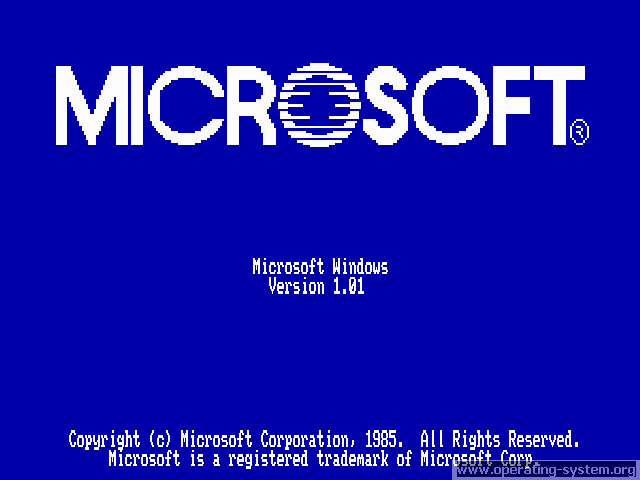
\includegraphics[scale=0.35]{img/win1.png}
\caption{Windows 1, Primer versión de interfaz gráfica}
\label{fig:dis1}
\end{figure}
Ciertamente Microsoft en toda su historia tiene alrededor de 23 versiones de su sistema operativo visibles a la luz publica, cada una de las versiones ha herede dado código de las versiones anteriores con mejoras en desempeño, administración de recursos, utilidades entre otras. A continuación se lista en orden ascendente la lista de Sistemas operativos y su versiones de acuerdo a lo mencionado en \fnurl{operating\-system.org}{http://www.operating-system.org}
\begin{multicols}{2}
    \begin{enumerate}
      \item MS-DOS
      \item Windows 
      \item Windows 1.0
      \item Windows 3.0
      \item Windows 3.11
      \item Windows 95
      \item Windows 98
      \item Windows CE
      \item Microsoft Auto
      \item Windows ME
      \item Windows NT 3.1
      \item Windows NT 4.0
      \item Windows NT Server 4.0
      \item Windows 2000
      \item Windows XP
      \item Windows Vista
      \item Windows Server 2003
      \item Windows Server 2008
      \item Windows Server 2012
      \item Windows Server 2016
      \item Windows 7
      \item Windows 8
      \item Windows 10
	\end{enumerate}
\end{multicols}
Entre las versiones destaco algunas de las caracteristicas mas relevantes y sus mejoras, estos datos fueron obtenidos gracias al proyecto \textbf{operating-system.org} 
$\\$
\texttt{\textbf{Windows1.0}}
\begin{itemize}
\item  Aplicaciones por defecto Paint, Calc, Write, Calendar, Notepad, Cardfile.
\end{itemize}
$\\$
\texttt{\textbf{Windows3.0}}
\begin{itemize}
\item  Mejoras en la ejecución del cooperative multitasking.
\item Implementacion para el direccionamiento de memorias de 32-bit en modo protegido.
\item Sistema Operativo de 16bits
\item El sistema de archivos maneja hasta 2 GB, y es FAT16. 
\end{itemize}
$\\$
$\\$
\texttt{\textbf{Windows3.11}}
\begin{itemize}
\item  Mejoras en la ejecución del cooperative multitasking.
\item Implementacion para el direccionamiento de memorias de 32-bit en modo protegido.
\item Sistema Operativo de 16bits
\item El sistema de archivos maneja hasta 2 GB, y es FAT16. 
\item Alta compatibilidad con versiones de DOS anteriores.
\end{itemize}

\texttt{\textbf{Windows95}}
\begin{itemize}
  \item  plug and play, para un gran numero de dispositivos.
  \item  Soporte en la cantidad de memoria ram.
  \item Implementacion de una interfaz ACPI para un modo de ahorro eléctrico. 
  \item El sistema de archivos maneja FAT32.
  \item compatible con procesadores X86.
  \item Cooperative multitasking solo para programas a 16bits.
  \item Bajos niveles de seguridad, escalabilidad en cuanto a recursos.
\end{itemize}
$\\$
\texttt{\textbf{Windows98}}
\begin{itemize}
\item  Implementacion de una librería para mejorar la administración de colores en monitores CRT. 
\item Plug and Play soportado para hardware como USB, Firewire IEEE 1394.
\item Implementacion oficial del sistema de archivos NTFS, ahora es posible acceder a particiones Linux ext2 con herramientas de terceros desde Windows98
\item  Soporte para DirectX 5.0, motor usado para realizar los renders de juegos. 
\end{itemize}
$\\$
\texttt{\textbf{WindowsNT}}
\begin{itemize}
\item  Implementacion de una librería para mejorar la administración de colores en monitores CRT. 
\item Soporte para múltiples protocolos de RED, se integran interfaces para el manejo de diferentes vendedores de hardware compatibles con el Standar UNIX-Linux.
\item Sistema de logueo de eventos del sistema. 
\item Arquitectura de Microkernel
\end{itemize}

\section{Gestión de Procesos, Memoria y Shell}
\subsection{Gestión de Procesos}
La administración de procesos es una de las partes integrales de cualquier sistema operativo moderno, dado que el sistema operativo debe reservar los recursos para los procesos, habilitar para su ejecución, compartir e intercambia datos con otros procesos. El sistema operativo también debe proteger esos recursos reservados y compartidos de los otros procesos sin afectar las demás actividades.
En el sistema operativo windows es posible realizar la administración de procesos utilizando diferentes utilidades.
Una de las herramientas presente en los sistemas operativos Microsoft Windows son \textbf{\textit{TASKLIST, TASKKILL}},ambos son los comandos que incluye la consola o interprete de comandos que Windows provee en su \textbf{cmd.exe}, aunque actualmente esta siendo reemplazado por un motor mucho mas poderoso que permite debugear de una manera mejor los scripts hechos en .NET, \textbf{PowerShell}. estas resultan muy útiles y nos auxilian cuando nos vemos en problemas a la hora de que un proceso necesite ser eliminado o gestionado. Podemos usarlos directamente en la consola de CMD o Símbolo del sistema, en archivos batch o en scripts, para administrar completamente los procesos y tareas ejecutándose en nuestro equipo. Podemos con ellos obtener información y crear listas detalladas, detener aplicaciones, tareas y procesos aun cuando están bloqueados y no responden. 
\begin{figure}[H]
 \centering
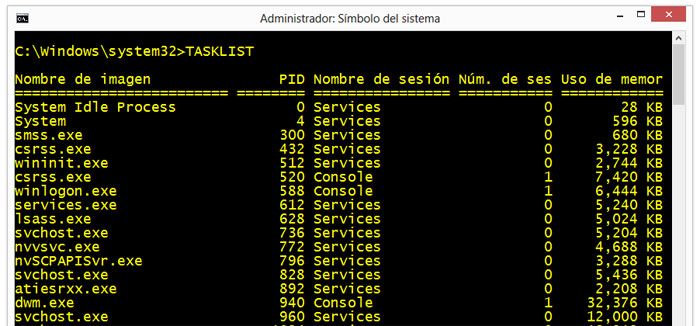
\includegraphics[scale=0.35]{img/task.jpg}
\caption{Windows cmd, Ejecución de Tasklist}
\label{fig:dis2}
\end{figure}
\subsection{Gestión de Memoria Windows}
Microsoft provee un sistema administrador de memoria en todos sus desarrollos, véase este \fnurl{link}{https://msdn.microsoft.com/en-us/library/windows/desktop/aa366525(v=vs.85).aspx} 

Cada proceso creado en el sistema operativo Windows de 32 y 64 bits generará su propio espacio de direcciones virtuales, es decir que podemos afirmar que todos los hilos de un proceso pueden acceder a su espacio de direcciones virtual, sin embargo los hilos de ese proceso no puede acceder a otras porciones de memoria de otros procesos por los mecanismos y esquemas de protección establecidos por Windows. Como es claro del link previo la memoria una vez que la maquina se encuentra encendida es dividida en dos secciones principalmente, la primera de ellas es el espacio de memoria que es necesario para que el kernel puede funcionar, es claro que esta zona en el sistema operativo tiene unos altos privilegios por lo que en general a partir de la versión Windows Vista, el kernel se encuentra protegido y oculto de los alcances del usuario a no ser de que se utilice una API apropiada con los permisos correspondientes. 

Por otra parte tenemos el espacio para la ejecución de las aplicaciones, obsérvese el siguiente esquema:
\begin{figure}[H]
 \centering
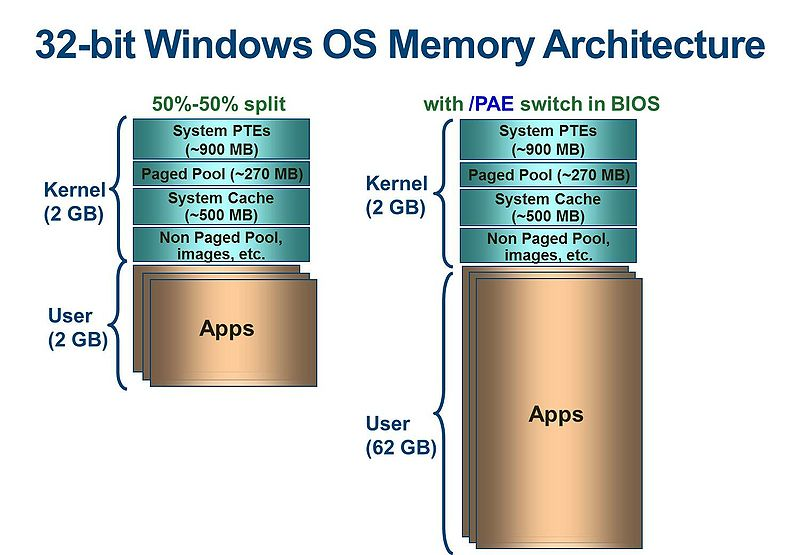
\includegraphics[scale=0.55]{img/winmemory.jpg}
\caption{Windows , División de memoria kernel vs user apps}
\label{fig:dis3}
\end{figure}
A su vez la sección de memoria del kernel se encuentra divida en varias secciones destinadas para el buen desempeño del kernel, entre ellas una tabla de paginas \fnurl{virtuales}{https://msdn.microsoft.com/en-us/library/windows/desktop/aa366912(v=vs.85).aspx} la cual es una estructura de datos interna para traducir la dirección virtual de ram a una ubicación física de la memoria. En una maquina presente con 4GB de memoria ram, esta sera divida en 2GB y 2GB correspondientes al kernel y al espacio de ejecución para las aplicaciones de usuario. 

\subsection{Gestión de Archivos}
Windows para la administración de archivos actualmente tiene \fnurl{componentes}{https://msdn.microsoft.com/en-us/library/windows/desktop/ee663264(v=vs.85).aspx} y servicios que soportan a las aplicaciones para acceder y almacenar datos. Los componentes son :
\begin{enumerate}
\item Sistema administrador de archivos
\item Acceso a Bases de datos
\item Soporte para la transferencia, sincronización y replicacion de datos.
\item Copias de segunda estancia. 
\end{enumerate}
En general el sistema de archivos tiene forma de árbol y formado por directorios, y los archivos contenidos en estos.

Las funciones del administrador de sistema de archivos son:
\begin{itemize}
\item Crear archivos
\item Eliminar  archivos
\item Compartir archivos para intercambiar información
\item Agrupar archivos en forma conveniente para el usuario
\item Respaldo y recuperación de la información
\item Acceso de los usuarios a la información sin necesidad de conocer la ubicación física.
\item Trabaja como interprete de comandos de manera amigable sin necesidad de usar programas de bajo nivel para comunicarse con el Sistema Operativo.
\end{itemize}
\section{Estructura del Sistema Operativo}
\begin{figure}[H]
 \centering
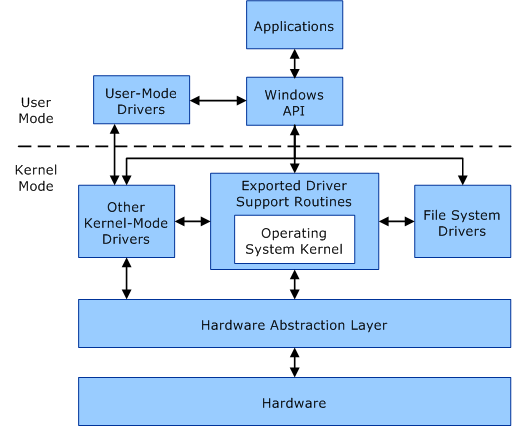
\includegraphics[scale=0.45]{img/windowsds.png}
\caption{Arquitectura del Sistema Operativo Windows, 10}
\label{fig:dis4}
\end{figure}
Todas las versiones de Windows han estado basadas en el Kernel con más de 20 años de edad, es el kernel de Windows NT,  La versión 5.1.2600 fue para la versión de Windows XP, la 6.0.6002 fue para Windows Vista, y la 6.1.7601 para Windows 7. actualmente la NT 10.0 es  el que utiliza Windows 10.Una de las principales características del Kernel de Windows NT es que es \textit{bastante modular}, y está basada en dos capas principales, la de usuario y la de kernel como se puede observar en la figura anterior (fig \ref{fig:dis4}). El sistema utiliza cada una para diferentes tipos de programa. Por ejemplo, las aplicaciones se ejecutan en el modo usuario, y los componentes principales del sistema operativo en el modo kernel. Mientras, la mayoría de los drivers suelen usar el modo kernel, aunque con excepciones.
Según la arquitectura que este tiene, Windows utiliza un Kernel híbrido, pero sobre todo también porque permite tener subsistemas en el espacio del usuario que se comunicaban con el kernel a través de un mecanismo de IPC, gracias a ello fue posible meter un subsistema que emulara completamente una miniversion de ubuntu en el denominado LSB.
\begin{figure}[H]
 \centering
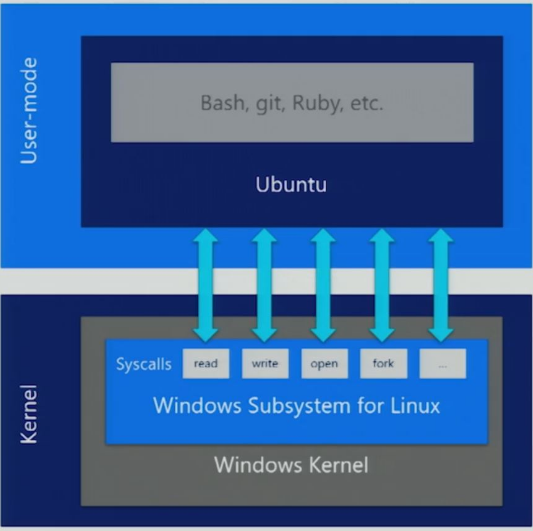
\includegraphics[scale=0.45]{img/ubuntu.png}
\caption{Windows, Linux Subsystem, Slides Oficiales}
\label{fig:dis5}
\end{figure}
\section{Clasificación del Sistema Operativo}
Según el libro de sistemas operativos de Los sistemas operativos pueden ser clasificados de acuerdo a :
\begin{itemize}
\item\textbf{Multiusuario}: Permite que dos o más usuarios utilicen sus programas al mismo tiempo. Algunos sistemas operativos permiten a centenares o millares de usuarios al mismo tiempo.
\item\textbf{Multiprocesador}: soporta el abrir un mismo programa en más de una CPU.
\item\textbf{Multitarea}: Permite que varios programas se ejecuten al mismo tiempo.
\item\textbf{Multitramo}: Permite que diversas partes de un solo programa funcionen al mismo tiempo.
\item\textbf{Tiempo Real}: Responde a las entradas inmediatamente. 
\end{itemize}
Windows actualmente soporta la gran mayoría de items descritos en el libro mencionado del señor Tanembaum(\textit{Ver caso de estudio Windows Vista})
\section{Administración de dispositivos de entrada y salida.}
Una computadora consiste de varios dispositivos que proveen una entrada y salida desde y para el mundo exterior, estos dispositivos pueden ser micrófonos, teclados, controladores de audio, disco duros, entre otros. Los controladores de cada dispositivo proveen el software que permite la conexión entre los dispositivos y el sistema operativo. La administración de dispositivos de entrada y de salida en Windows es realizada gracias a el I/O \fnurl{Manager}{https://docs.microsoft.com/en-us/windows-hardware/drivers/kernel/windows-kernel-mode-i-o-manager} este se encarga de administrar la conexión entre las aplicaciones y las interfaces provistas por los drivers de cada dispositivo, esta comunicacion es hecha principalmente a través de unos paquetes de conexión, IRPs similares a los paquetes de red pero interpretados por el administrador. Técnicas de programación como la programación \fnurl{Sincrona y Asincrona}{https://docs.microsoft.com/en-us/windows-hardware/drivers/kernel/general-i-o-programming-techniquesv} son usadas para una buen manejo de las peticiones. 
\section{Manejo de Interrupciones}
Para tener una claridad frente al manejo de interrupciones en el sistema operativo Windows, es necesario tener claridad que es una interrupción. 
De la consulta realizada una interrupción avisa al procesador de que tiene una tarea de máxima prioridad requiriendo que se interrumpa el código que se esté procesando ahora mismo en el procesador. Entonces el procesador suspende dicha actividad, guarda su estado, y ejecuta una función llamada gestor de interrupciones para gestionar el caso. Con la nueva solicitud y tan pronto terminamos se envía la señal de continuar. Cuando el gestor de interrupciones ha terminado su trabajo, el procesador continúa desde el punto que se quedó con el proceso que estaba en ejecución.
\section{Referencias}
\hyperref[http://www.nareshmdr.com.np/ictexams/?p=139]{http://www.nareshmdr.com.np/ictexams/?p=139}
$\\$
\hyperref[http://histinf.blogs.upv.es/2011/01/03/historia-de-microsoft/]{http://histinf.blogs.upv.es/2011/01/03/historia-de-microsoft/}
$\\$
\hyperref[https://www.genbeta.com/a-fondo/como-es-el-kernel-de-windows-y-cuales-son-sus-diferencias-con-el-de-linux, diferencias entre el kernel de Windows y Linux, Genbeta]{https://www.genbeta.com/a-fondo/como-es-el-kernel-de-windows-y-cuales-son-sus-diferencias-con-el-de-linux}

\end{document}